\scanpage{3}

\diagram{\resizebox{\linewidth}{!}{{\small\setlength{\arraycolsep}{3pt}
$\begin{array}{ccc|l@{\quad}l}
V_1&V_2&V_3&V_1\ \text{\unsure{borde|bords}}\ \Gamma'_2,\Gamma'_3&
\Gamma'_1\ \text{bordé par}\ V_2,V_3\\
\overset{\deleted{\unsure{\circ|\bullet}}}{\Gamma}''_1&
\overset{\deleted{\circ}}{\Gamma}''_2&
\overset{\deleted{\circ}}{\Gamma}''_3&
V_2\ \text{borde}\ \Gamma'_3,\Gamma'_1&\Gamma'_2\ \text{---}\ V_3,V_1\\
\shortparallel&\shortparallel&\shortparallel&&\\[-.4ex]
\Gamma'_1-\partial&\Gamma'_2-\partial&\Gamma'_3-\partial&
V_3\ \text{borde}\ \Gamma'_1,\Gamma'_2&\Gamma'_3\ \text{---}\ V_1,V_2
\end{array}$}}}

\[
\partial=\{\unsure{x},y\}
\]

\[
\begin{aligned}
\Gamma_1&=\Gamma_2\cup\Gamma_3=\Gamma'_{\unsure{2|1}}\cup\Gamma'_3
=\Gamma''_1\cup\Gamma''_2\cup\partial\\
\Gamma_2&=\Gamma_3\cup\Gamma_1=\Gamma'_3\cup\Gamma'_1
=\Gamma''_3\cup\Gamma''_1\cup\unsure{\dot\partial|\partial}\\
\Gamma_3&=\Gamma_1\cup\Gamma_2=\Gamma'_1\cup\Gamma'_2
=\Gamma''_1\cup\Gamma''_2\cup\partial
\end{aligned}
\]

\noindent\begin{minipage}[c]{.34\linewidth}
% The lettering in the drawing is turned a quarter turn on the sheet.
\figure{\resizebox{\linewidth}{!}{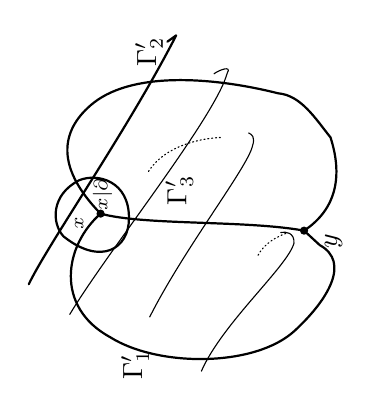
\begin{tikzpicture}[x=.8cm,y=.8cm,line cap=round,line join=round]
\begin{scope}[rotate=90]
\draw[thick] (0,1.25) .. controls (-.51,1.83) and (-1.48,1.98) .. (-1.96,1.10)
 .. controls (-2.44,.34) and (-2.44,-1.20) .. (-1.86,-1.83)
 .. controls (-1.37,-2.36) and (-.77,-2.72) .. (-.50,-2.23) -- (-.27,-1.98);
\draw[thick] (0,1.25) .. controls (.79,2.02) and (1.37,1.85) .. (1.76,1.36)
 .. controls (2.29,.68) and (2.14,-.66) .. (1.91,-1.57)
 .. controls (1.88,-1.93) and (1.51,-2.16) .. (1.21,-2.40)
 .. controls (.62,-2.59) and (.08,-2.51) .. (-.27,-1.98);
\draw[thick] (0,1.25) .. controls (-.19,.56) and (-.10,-1.05) .. (-.27,-1.98);
\draw[thick] (-.36,1.84) .. controls (-.84,1.24) and (-.55,.80) .. (-.08,.80)
 .. controls (.52,.79) and (.65,1.30) .. (.53,1.59) .. controls (.30,2.04) and (-.15,2.03) .. cycle;
\draw[thick] (-1.12,2.39) .. controls (-.49,2.09) and (1.36,.80) .. (2.83,.05) -- (2.73,.19);
\draw (-1.60,1.74) .. controls (-.60,1.14) and (1.53,-.57) .. (2.23,-.76) .. controls (2.36,-.84) and (2.28,-.63) .. (2.22,-.55);
\draw (-1.64,.47) .. controls (-.55,-.08) and (.73,-1.08) .. (1.07,-1.16) .. controls (1.22,-1.21) and (1.26,-1.15) .. (1.28,-1.10);
\draw (-2.50,-.35) .. controls (-1.73,-.69) and (-.85,-1.71) .. (-.47,-1.82) .. controls (-.30,-1.83) and (-.28,-1.69) .. (-.30,-1.61);
\draw[densely dotted] (.67,.49) .. controls (1.09,.22) and (1.20,-.36) .. (1.21,-.68);
\draw[densely dotted] (-.66,-1.25) .. controls (-.47,-1.35) and (-.36,-1.55) .. (-.30,-1.73);
\fill (0,1.25) circle (.065); \fill (-.27,-1.98) circle (.065);
\node[rotate=90] at (-2.40,.70) {$\Gamma'_1$};
\node[rotate=90] at (2.57,.48) {$\Gamma'_2$};
\node[rotate=90] at (.37,.00) {$\Gamma'_3$};
\node[rotate=90,inner sep=0pt] at (-.16,1.59) {\scriptsize $x$};
\node[rotate=90,inner sep=0pt] at (.31,1.22) {\scriptsize $\deleted{\unsure{x|\partial}}$};
\node[rotate=90] at (-.44,-2.45) {$y$};
\end{scope}
\end{tikzpicture}}}
\end{minipage}\hfill
\begin{minipage}[c]{.64\linewidth}
\[
\resizebox{\linewidth}{!}{$\displaystyle
\Gamma_3^{\deleted{\unsure{\circ|'}}}=\Gamma''_1\cup\Gamma''_{\unsure{2|1}}\cup\partial
\ \big|\quad U_3=V_1\cup V_2\cup\Gamma''_3\quad\big|\quad V_3$}
\]

\[
\dot U_3=\Gamma_3\qquad U_3\cup
\]
\end{minipage}

\[
\unsure{\cdot}\ U,C,V
\]
% archive sheet number: 2
